\newpage
\section{Large area device simulation}
Gpvdm primerally focuses on drift diffusion modeling of small area device such as solar cells and OFETs.

\label{ref:la}

\begin{figure}[H]
\centering
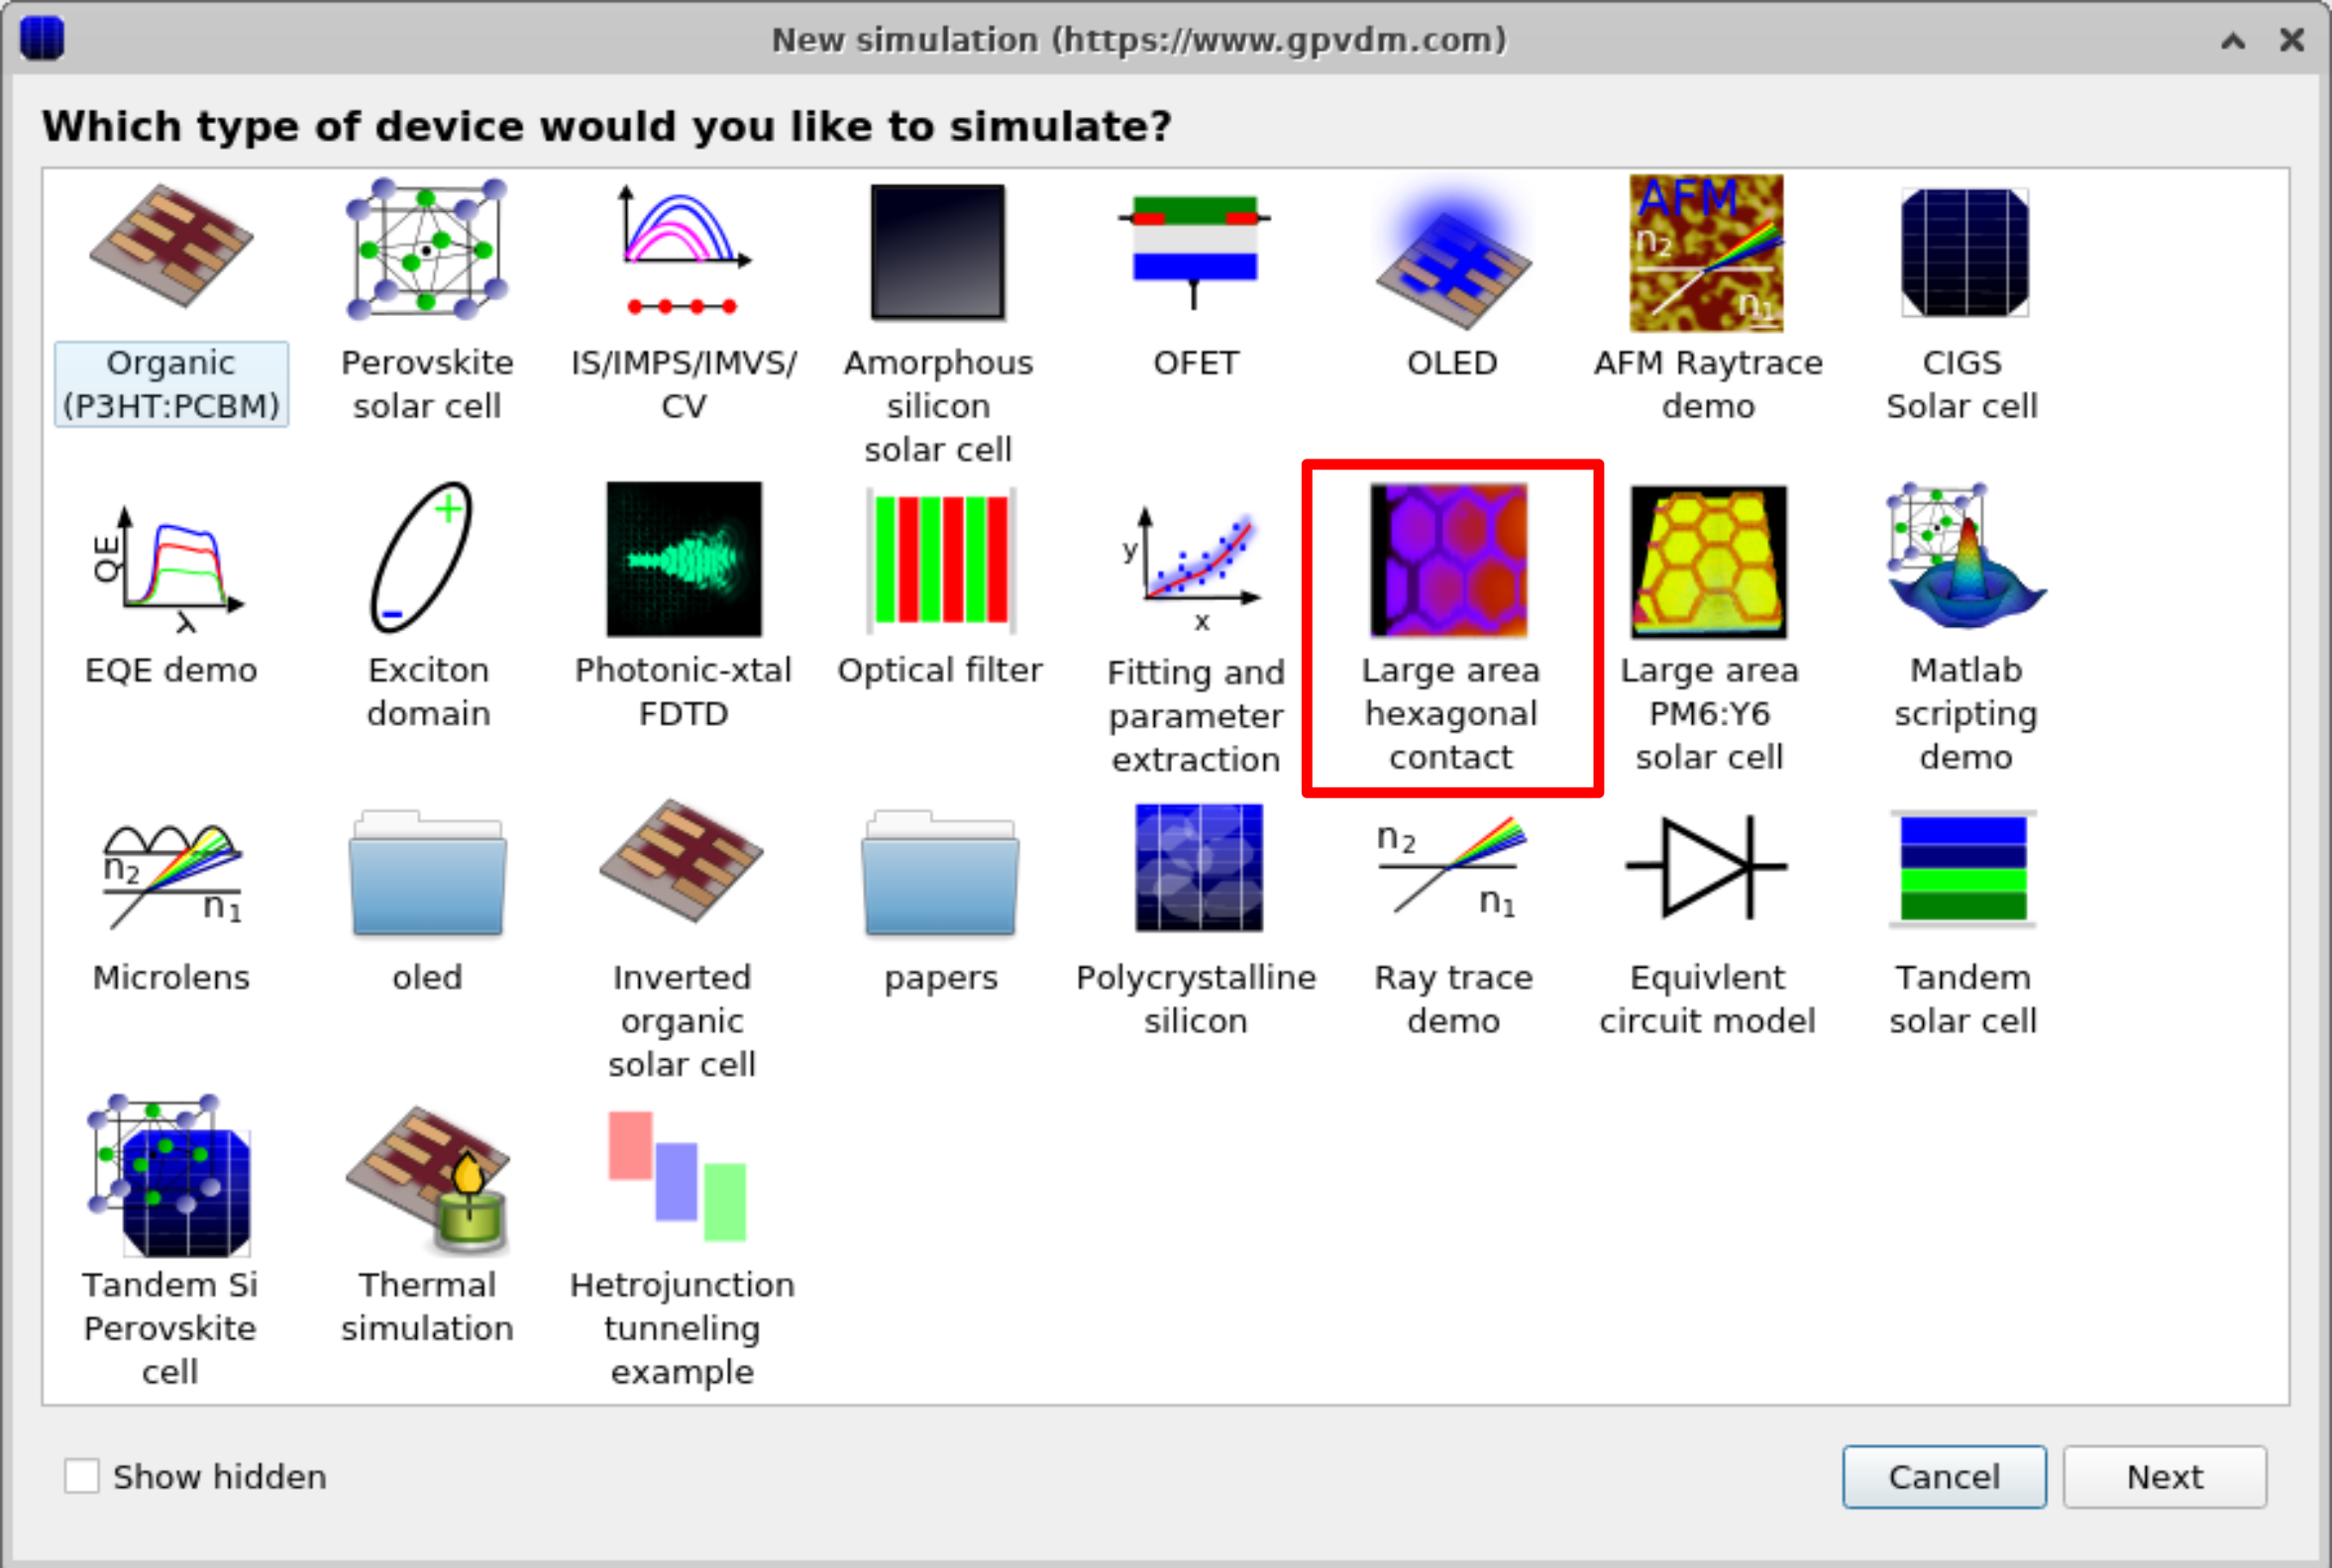
\includegraphics[width=\textwidth]{./images/la_0.png}
\caption{A 1D diagram of the mesh}
\label{fig:emeshdiagram}
\end{figure}

\begin{figure}[H]
\centering
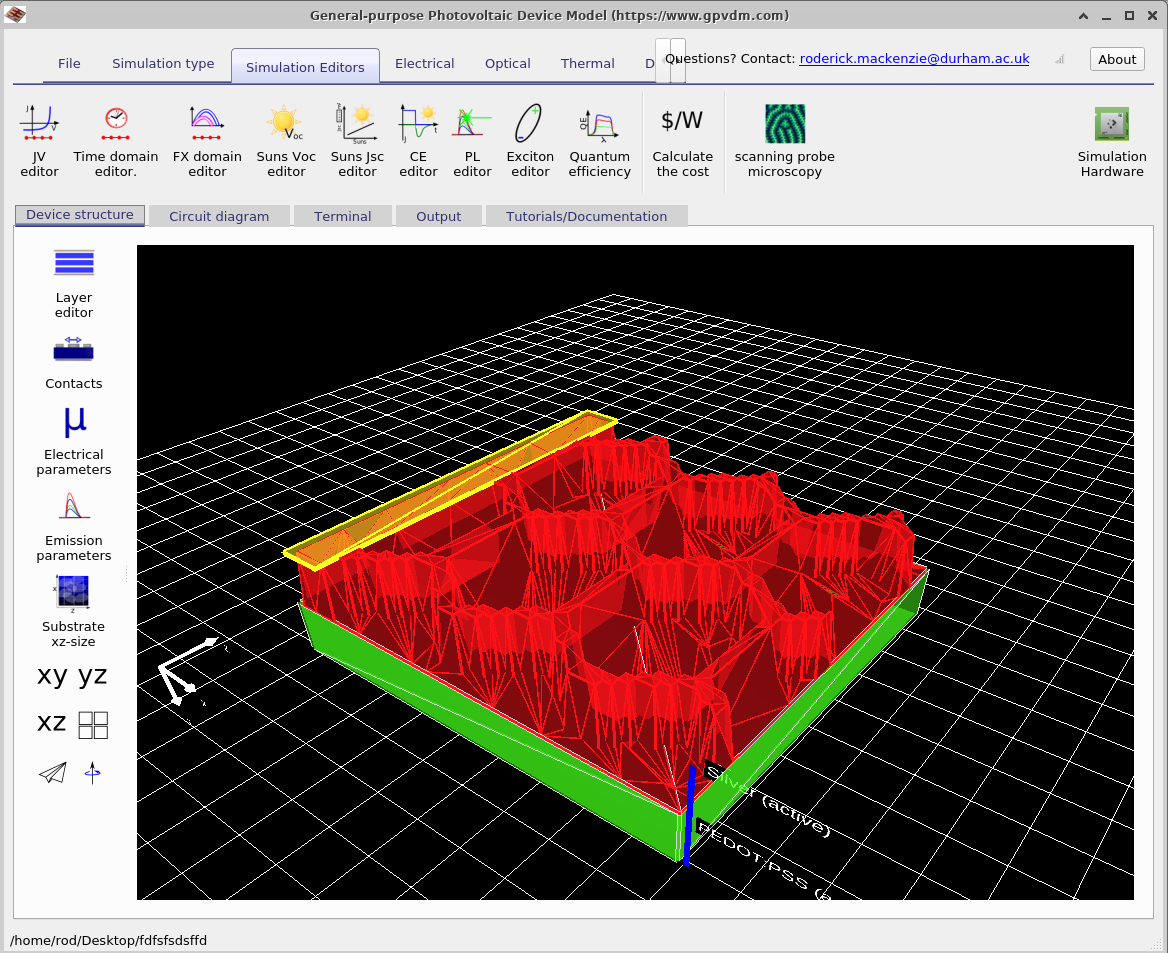
\includegraphics[width=\textwidth]{./images/la_1.png}
\caption{A 1D diagram of the mesh}
\label{fig:emeshdiagram}
\end{figure}

\begin{figure}[H]
\centering
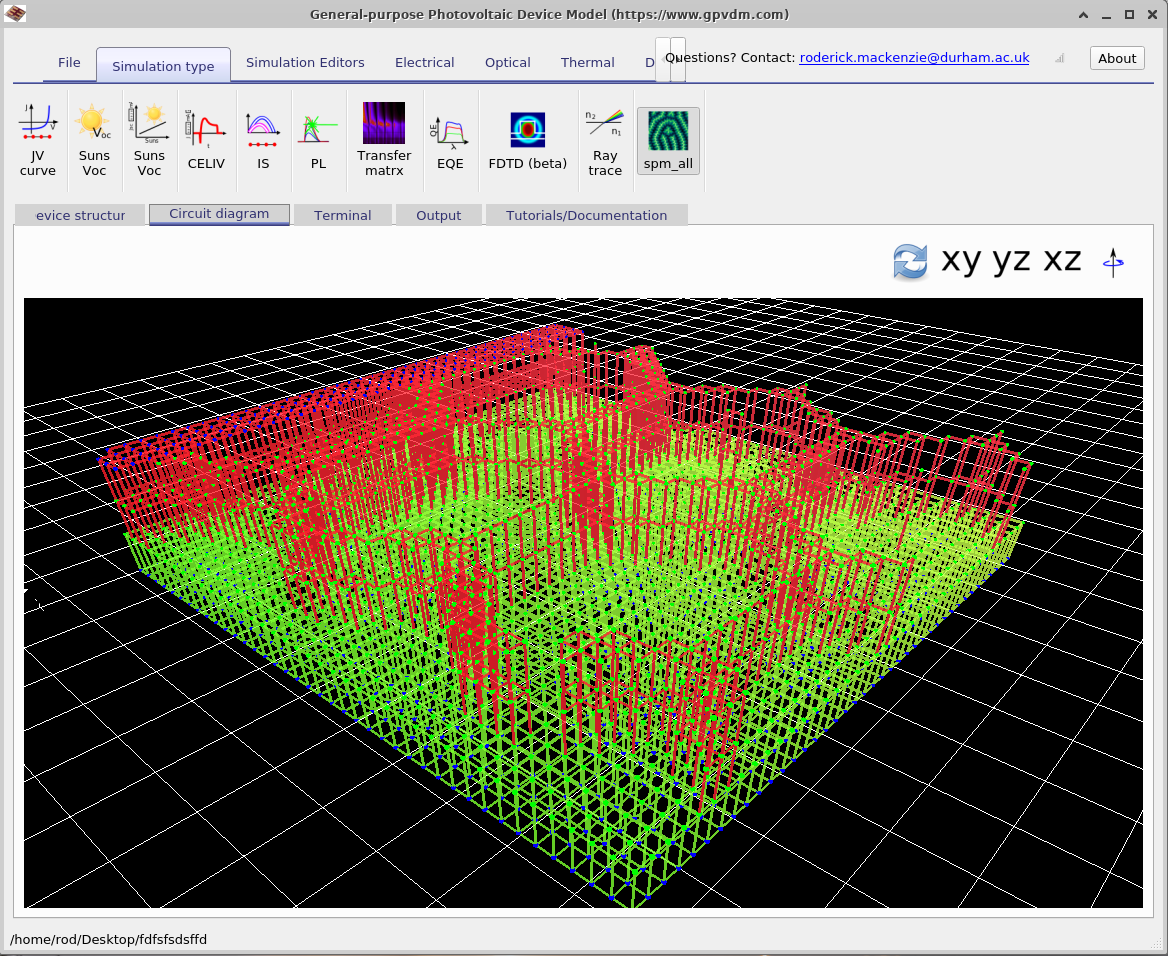
\includegraphics[width=\textwidth]{./images/la_2.png}
\caption{A 1D diagram of the mesh}
\label{fig:emeshdiagram}
\end{figure}

\begin{figure}[H]
\centering
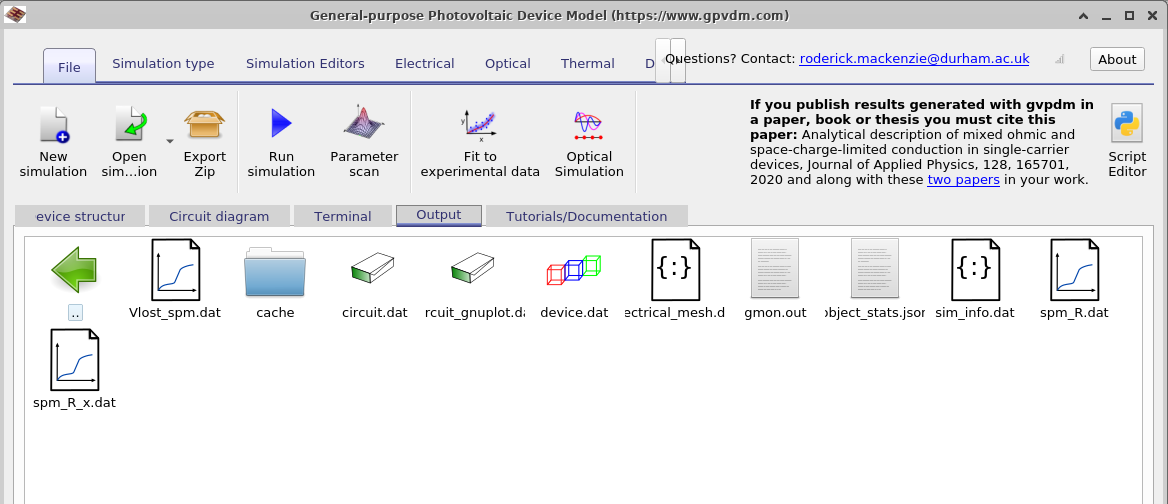
\includegraphics[width=\textwidth]{./images/la_3.png}
\caption{A 1D diagram of the mesh}
\label{fig:emeshdiagram}
\end{figure}

\begin{figure}[H]
\centering
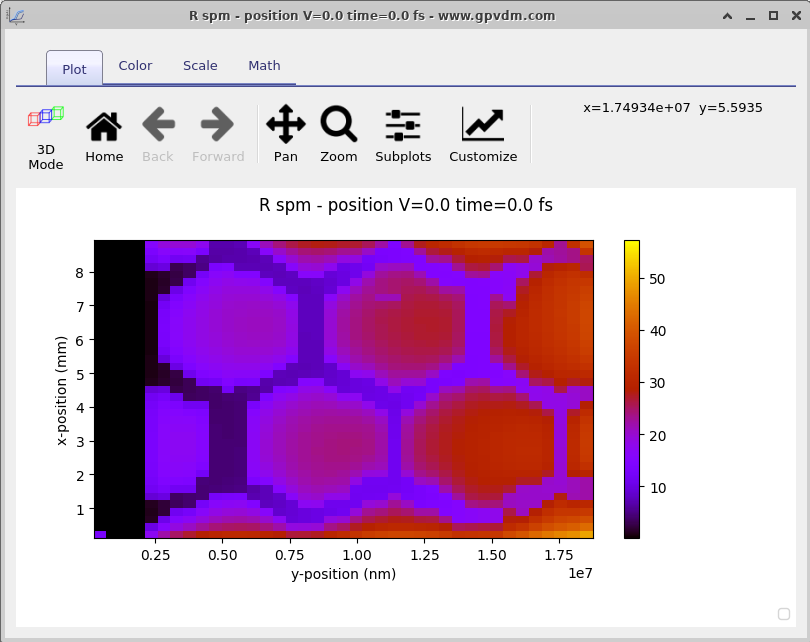
\includegraphics[width=\textwidth]{./images/la_4.png}
\caption{A 1D diagram of the mesh}
\label{fig:emeshdiagram}
\end{figure}

\begin{figure}[H]
\centering
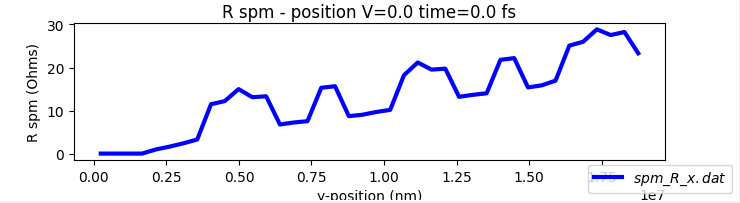
\includegraphics[width=\textwidth]{./images/la_5.png}
\caption{A 1D diagram of the mesh}
\label{fig:emeshdiagram}
\end{figure}

\begin{figure}[H]
\centering
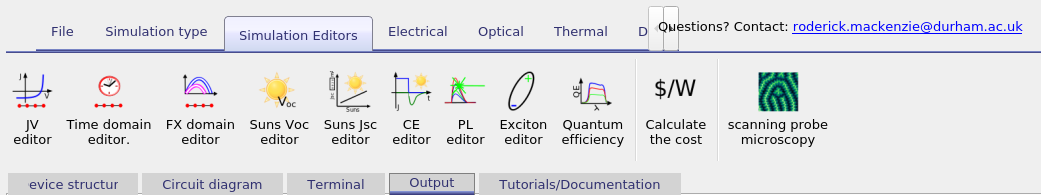
\includegraphics[width=\textwidth]{./images/la_6.png}
\caption{A 1D diagram of the mesh}
\label{fig:emeshdiagram}
\end{figure}

\begin{figure}[H]
\centering
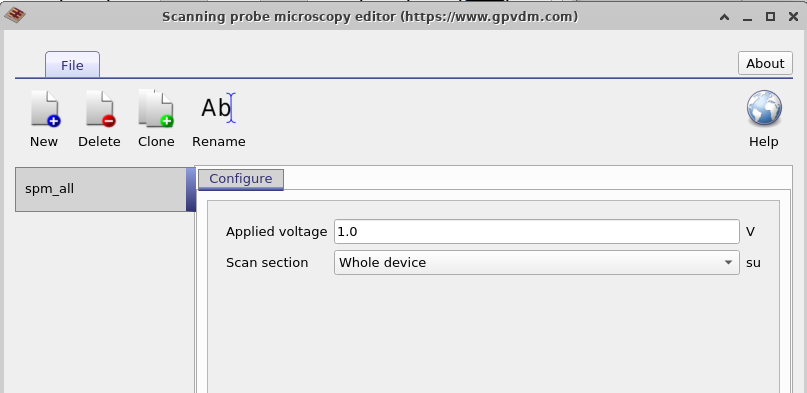
\includegraphics[width=\textwidth]{./images/la_7.png}
\caption{A 1D diagram of the mesh}
\label{fig:emeshdiagram}
\end{figure}


\begin{table}[H]
\begin{center}
\begin{tabular}{ |c|c|c| } 
 \hline
	Device type			& 	Number of dimentions  \\ 
 \hline
	$Solar cells$ 		&	1D \\ 
	$Optical filter$	&	1D\\ 
	$OFET$ 				&	2D\\ 
 \hline
\end{tabular}
\caption{How many dimensions should I use to simulate my device.}
\end{center}
\end{table}

